\documentclass[oneside]{book}

%TODOTODOTODOTODOTODOTODOTODOTODOTODOTODOTODOTODOTODOTODOTODOTODOTODOTODO
%juiste git commit voorzien!!!

% Load the VUB package.
% This has many options, please read the documentation at
% https://gitlab.com/rubdos/texlive-vub
\usepackage{vub}

% Some highly suggested packages, please read their manuals.
\usepackage{cleveref}
\usepackage[natbib,style=apa]{biblatex}
\addbibresource{../bibliography.bib}

%space between paragraph and indent all
\setlength{\parskip}{1em}
\usepackage{indentfirst}

%space between bib entries
\setlength\bibitemsep{2\itemsep}

%images settings
\graphicspath{ {./images/} }
\usepackage{graphicx,caption}
\usepackage{float}
\usepackage{rotating}
\usepackage{tikz}

%fix section numbering for use with parts
\renewcommand*\thepart{\Roman{part}}
\makeatletter
\@addtoreset{section}{part}
\makeatother
\renewcommand*\thesection{\arabic{part}.\arabic{section}}
\renewcommand*\thesubsection{\thesection.\arabic{subsection}}

%START title
% done
\title{Animal classification AI}
\subtitle{Machine Learning}
\author{Lennert Bontinck}
\date{January, 2021}
\promotors{Master Computer Science: AI}
\faculty{Sciences and Bio-Engineering Sciences}
\begin{document}
\frontmatter
\maketitle
%END title


%START abstract
% done
\chapter*{Abstract}

This report documents the development of an \textit{animal classification AI} using a more \textit{old-school approach} of Visual-Bag-of-Words models.
This AI is capable of differentiating 12 different animals.
These models, and thus the AI, are developed in Python-based Jupyter Notebooks accompanied by this document.
This animal classification AI was developed as a fulfilment of the Machine Learning course requirements and was used to compete in the organised Kaggle competition \citep{kaggle_competition}.

Part \ref{part:about_the_code} of this report discusses the accompanied code in general.
Section \ref{section:inc_files} explains which files are the most important. 
Section \ref{section:ideology_dev_code} describes the ideology used to created the code. 
To make testing multiple models easier, \textit{a template} for model exploration was created and is discussed in section \ref{section:typical_model_exploration}.

In part \ref{part:data_analysis}, the \textit{data analysis} part of this project is discussed.
Section \ref{section:DA_data_distribution} talks about the \textit{unbalanced data} distribution.
In the next section, section \ref{section:DA_deeper_look_data}, a deeper look is taken into the data and possible \textit{preprocessing} is discussed.
The last few sections of this part discuss how the \textit{feature extraction} is dealt with and what the numerical representation looks like.

The \textit{linear baseline model} is discussed in part \ref{part:linear_baseline}.
This model is a fine-tuned \textit{Logistic Regression model} from the SciKit Learn library.
This model is often used to compare other models with.
Only models that perform better then this baseline model should be considered.
This part discusses the parameters used and the road to finding those optimal parameters.

Afterwards \textit{Support vector Classifiers} (SVC) are explored.
Part \ref{part:svc} discusses non-linear SVC models with different kernels and finds the \textit{rbf kernel} to be the best from three tested kernels.
Part \ref{part:linear_svc} focuses on linear SVC models in a similar fashion and finds them to perform worse.
An ensemble approach is discussed in part \ref{part:gradien_boost}.
This approach makes use of Gradient Boosting which, while interesting, didn't perform well.

It is chosen to do the model analysis in a separate part, part \ref{part:model_anal}.
Afterwards, part \ref{part:final_model} goes over some other possible optimisations considering what is learned from all experiments thus far.
Some of these are implemented whilst others are just discussed in a theoretical manner.
This results in the final, best performing, model.
Afterwards, in part \ref{part:conclusion}, a short conclusion is given.

It is noted that the page count of this document doesn't represent its actual length due to clear part separation from the used template and large figures.
Content that isn't crucial or is a repetition of supplied information is discarded or given as an appendix.
%END abstract


%TOC
\tableofcontents
\mainmatter

%START about
\part{About the code}
\label{part:about_the_code}

%------------------------------------

\section{Files accompanied by this report}
\label{section:inc_files}
Since this report discusses the development of an AI, \textit{a lot of code} is discussed as well.
This code is not shown inside this document but is available on the GitHub repository \citep{github_project}.
All code is written in Python-based Jupyter Notebooks.

%------------------------------------


\section{Ideology of the developed code}
\label{section:ideology_dev_code}
The Jupyter Notebooks have many inline comments and markdown blocks to make reading the code easier.
If code is extensively discussed in this report, a reference to the corresponding section is made inside the code. 
Some of the gathered results come from time-consuming function calls.
These can take \textit{multiple hours} to complete.
To spare some time, these results are saved in a Pickle file so they can be loaded in without having to do the function call.
The Notebooks are written in a way that makes testing multiple models easy, paying extra attention to reusability. 

%------------------------------------

\section{A typical model exploration}
\label{section:typical_model_exploration}
The testing of a model consists of two main parts.
Firstly the input of the model has to be optimized.
Afterwards, the (hyper)parameters of the model itself can be optimized.
These steps are clearly visible with the discussed models in this report since they follow a form of \emph{template}.
This template makes testing new models rather easy.
After optimizing everything in a standalone fashion, it has to be checked that these newly optimized parameters do not influence previously optimized parameters.
The resulting model should perform better than the linear baseline model in order to be considered.
Whilst many abstractions were made and creating a \emph{one-call pipeline} is possible, it's chosen to not do so.
This is because \textit{human reasoning} can be required in finding truly optimal parameters.
It also makes understanding and discussing the model easier.
After all, the goal of this report is to gather an understanding on how these models work, not solely  to get the best Kaggle score.

%------------------------------------


\section{Technical remarks}
\label{section:technical_remarks}

Most source files, for this report and the created models, are available on GitHub \citep{github_project}. Some files, like the used training images, were not included in this GitHub repository. Details about this can be found on the GitHub page (\texttt{README} file). Rights to this GitHub repository can be asked from the author. This report was created in \LaTeX{} by modifying the VUB themed template from Ruben De Smet (\citeyear{latex_template}).

%START what's next
\part{What's next}
\label{part:whats_next}

%------------------------------------

\section{Further development}
\label{section:further_development}

Due to limited time available, this intermediate report and the current state of the project isn't overwhelming in any stretch of the imagination.
Because of this, a special thanks is given to the teacher and teaching assistants who've softened the requirements for the intermediate report.

In the time available until the final deadline many new possibilities for creating a better model will be explored, this might include but is not limited to:
\begin{itemize}
    \item Preprocessing can be explored.
    \item More available models need to be tested and compared to the linear baseline model.
    \item Nesting multiple good performing models might be an option, using weighted probabilities.
\end{itemize}

Some aspects of the created models and pipeline might also be modified further once the open issues discussed in section \ref{section:open_issues} are resolved.

%------------------------------------

\section{Open issues}
\label{section:open_issues}

While developing the first models many questions arose. Most are already answered by googling or discussion with colleagues. Open questions that are not yet answered are listed below, for which guidance from the teaching assistants is asked.

\begin{itemize}
    \item The data is not available as a pickle file for the SURF descriptor.
\end{itemize}

%START figures
\chapter*{More figures}
\addcontentsline{toc}{chapter}{More figures}

Some figures are referred to in the text but not placed directly under the text. These are included in this list. All figures are high resolution thus zooming in the PDF should be viable to get a clearer view.

%------------------------------------

\section*{Overview of training set}

\begin{figure}[H]
    \begin{center}
        \fbox{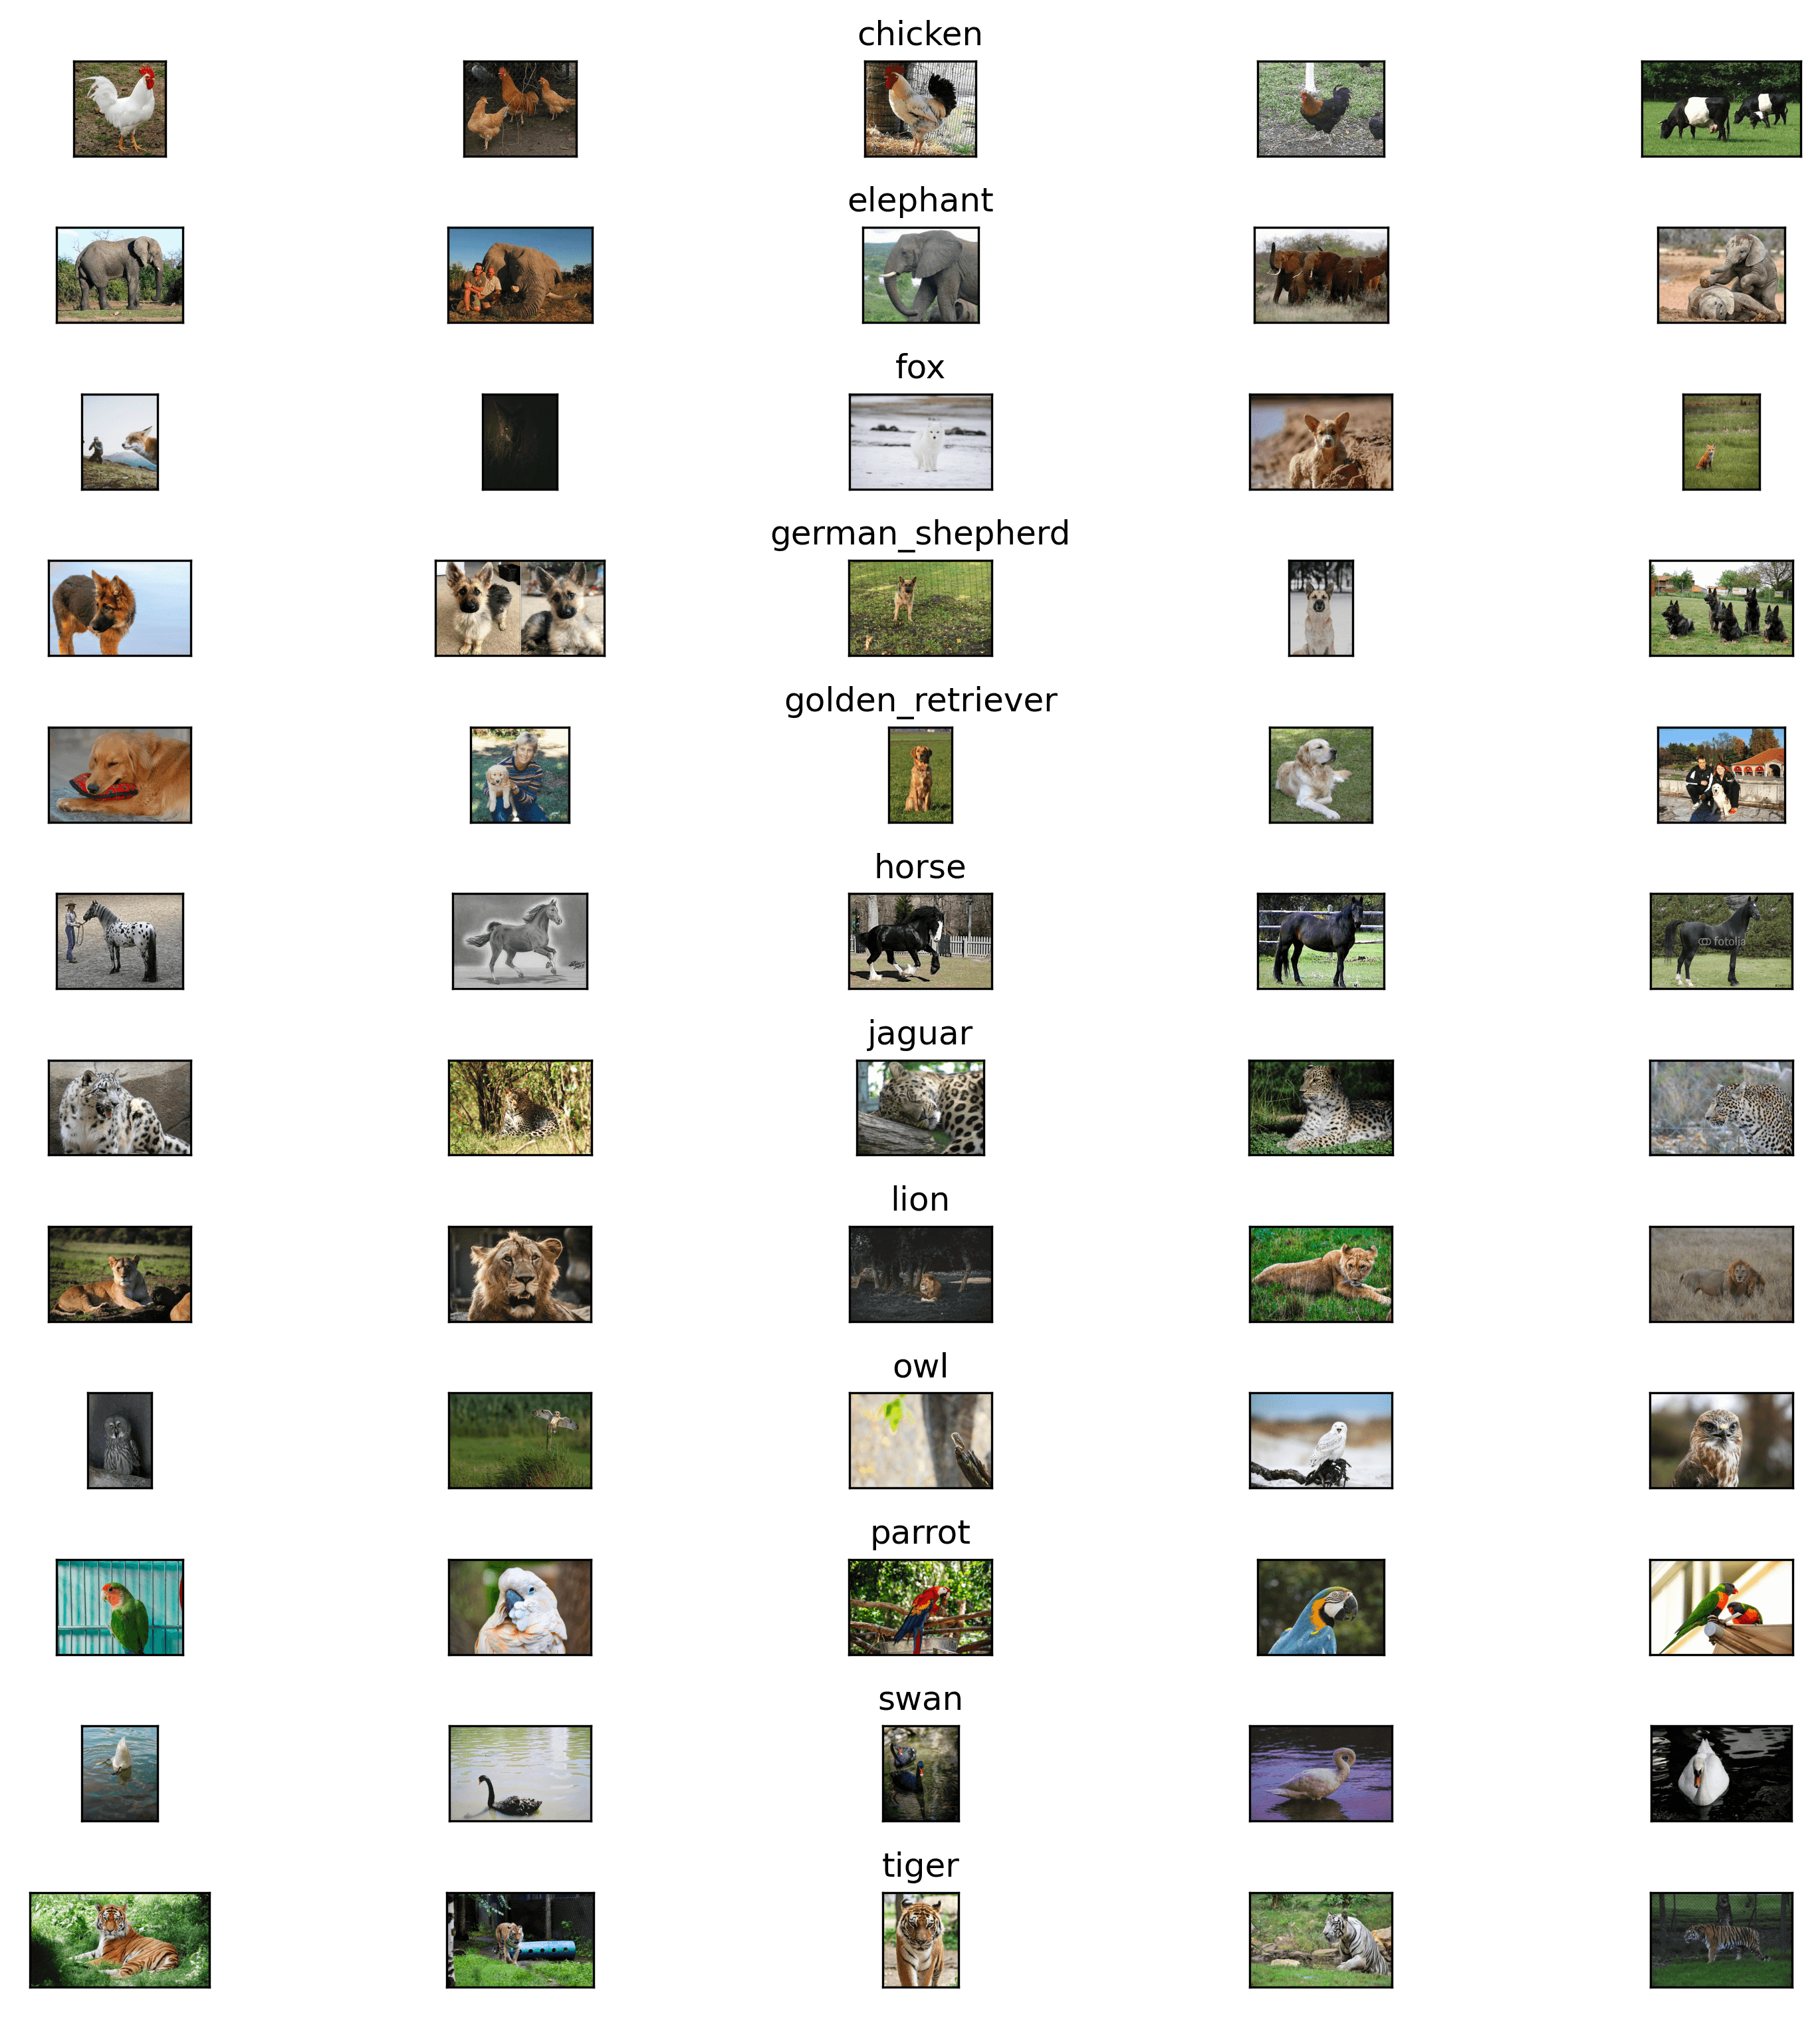
\includegraphics[width=0.70\linewidth]{images/1-data_analysis-labeled_data_overview.png}}
    \end{center}
    \captionsetup{width=0.65\linewidth}
    \captionsetup{justification=centering}
    \caption{An overview of the supplied data per class.}
    \label{fig:1-data_analysis-labeled_data_overview.png}
\end{figure}

%------------------------------------

\section*{Overview of features data}

\begin{figure}[H]
    \fbox{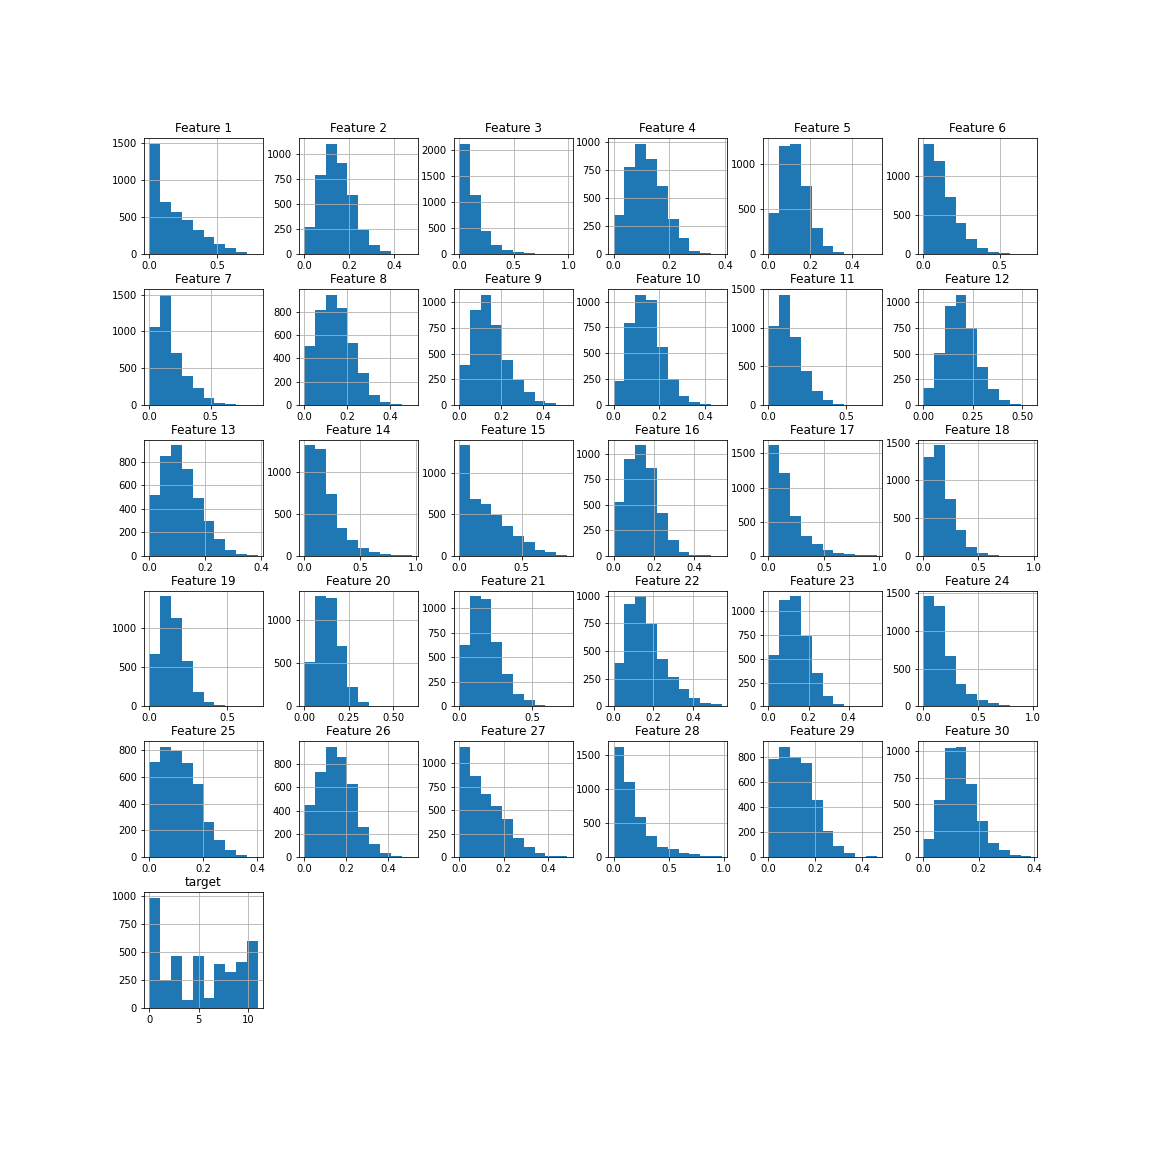
\includegraphics[width=1\linewidth]{images/1-data_analysis-feature_representation.png}}
    \captionsetup{width=0.85\linewidth}
    \captionsetup{justification=centering}
    \caption{An overview of the first 30 features data from a SIFT descriptor.}
    \label{fig:1-data_analysis-feature_representation}
\end{figure}

%------------------------------------

\section*{Linear baseline model - input optimisation (small)}

\begin{figure}[H]
  \centering
  \begin{minipage}[b]{0.4\textwidth}
    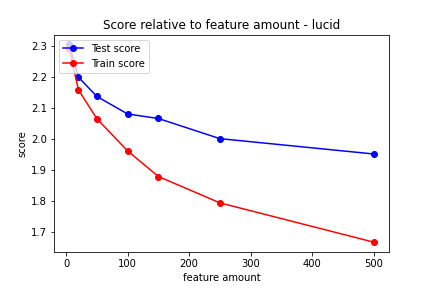
\includegraphics[width=\textwidth]{images/2-LBM-feature_amount_lucid_small_values.png}
  \end{minipage}
  \hfill
  \begin{minipage}[b]{0.4\textwidth}
    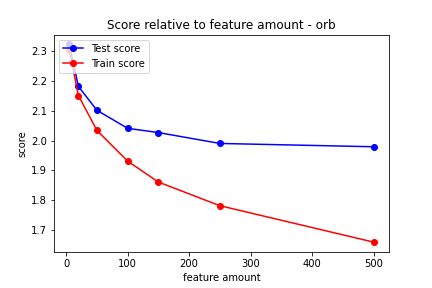
\includegraphics[width=\textwidth]{images/2-LBM-feature_amount_orb_small_values.png}
  \end{minipage}
\end{figure}

\begin{figure}[H]
  \centering
  \begin{minipage}[b]{0.4\textwidth}
    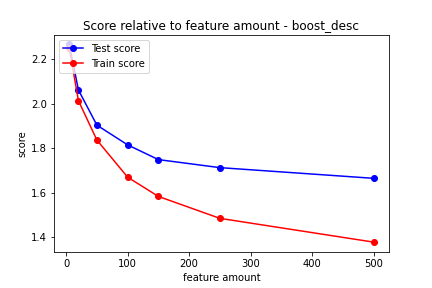
\includegraphics[width=\textwidth]{images/2-LBM-feature_amount_boost_desc_small_values.png}
  \end{minipage}
  \hfill
  \begin{minipage}[b]{0.4\textwidth}
    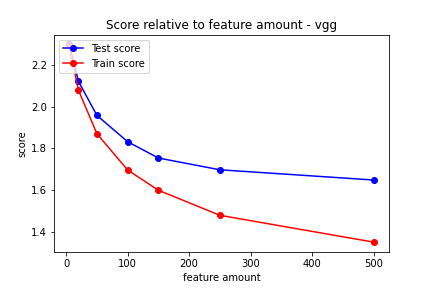
\includegraphics[width=\textwidth]{images/2-LBM-feature_amount_vgg_small_values.png}
  \end{minipage}
\end{figure}

\begin{figure}[H]
  \centering
  \begin{minipage}[b]{0.4\textwidth}
    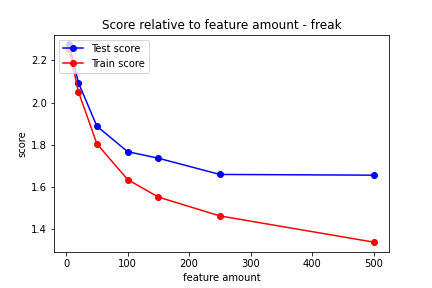
\includegraphics[width=\textwidth]{images/2-LBM-feature_amount_freak_small_values.png}
  \end{minipage}
  \hfill
  \begin{minipage}[b]{0.4\textwidth}
    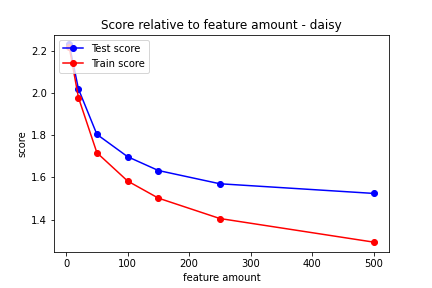
\includegraphics[width=\textwidth]{images/2-LBM-feature_amount_daisy_small_values.png}
  \end{minipage}
\end{figure}

\begin{figure}[H]
  \centering
  \begin{minipage}[b]{0.4\textwidth}
    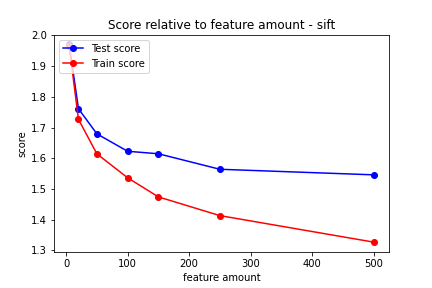
\includegraphics[width=\textwidth]{images/2-LBM-feature_amount_sift_small_values.png}
  \end{minipage}
\end{figure}

%------------------------------------

\section*{Linear baseline model - input optimisation (large)}

\begin{figure}[H]
  \centering
  \begin{minipage}[b]{0.4\textwidth}
    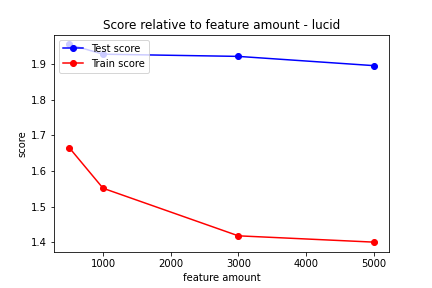
\includegraphics[width=\textwidth]{images/2-LBM-feature_amount_lucid_large_values.png}
  \end{minipage}
  \hfill
  \begin{minipage}[b]{0.4\textwidth}
    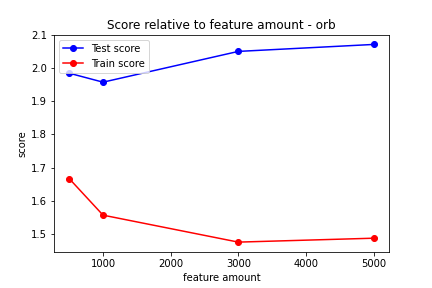
\includegraphics[width=\textwidth]{images/2-LBM-feature_amount_orb_large_values.png}
  \end{minipage}
\end{figure}

\begin{figure}[H]
  \centering
  \begin{minipage}[b]{0.4\textwidth}
    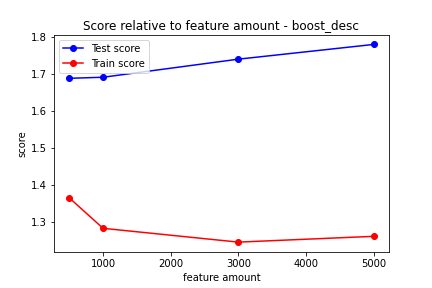
\includegraphics[width=\textwidth]{images/2-LBM-feature_amount_boost_desc_large_values.png}
  \end{minipage}
  \hfill
  \begin{minipage}[b]{0.4\textwidth}
    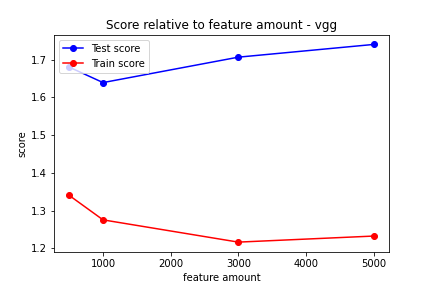
\includegraphics[width=\textwidth]{images/2-LBM-feature_amount_vgg_large_values.png}
  \end{minipage}
\end{figure}

\begin{figure}[H]
  \centering
  \begin{minipage}[b]{0.4\textwidth}
    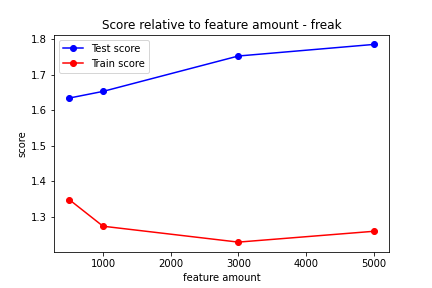
\includegraphics[width=\textwidth]{images/2-LBM-feature_amount_freak_large_values.png}
  \end{minipage}
  \hfill
  \begin{minipage}[b]{0.4\textwidth}
    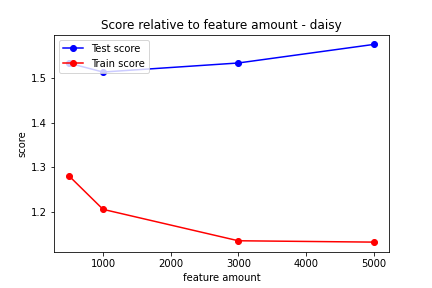
\includegraphics[width=\textwidth]{images/2-LBM-feature_amount_daisy_large_values.png}
  \end{minipage}
\end{figure}

\begin{figure}[H]
  \centering
  \begin{minipage}[b]{0.4\textwidth}
    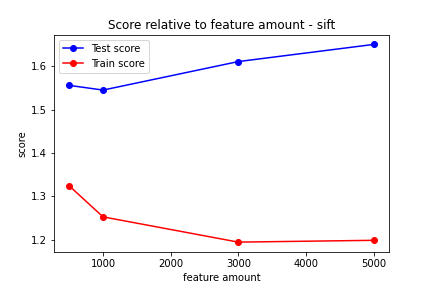
\includegraphics[width=\textwidth]{images/2-LBM-feature_amount_sift_large_values.png}
  \end{minipage}
\end{figure}

%------------------------------------

\section*{Linear baseline model - optimal DAISY}

\begin{figure}[H]
    \fbox{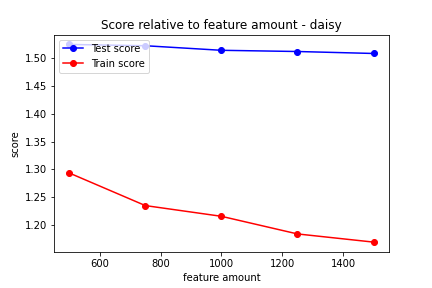
\includegraphics[width=1\linewidth]{images/2-LBM-feature_amount_daisy_daisy_optimal.png}}
    \captionsetup{width=0.85\linewidth}
    \captionsetup{justification=centering}
    \caption{An extra test for finding the optimal feature amounts for the DAISY descriptor.}
    \label{fig:2-LBM-feature_amount_daisy_daisy_optimal}
\end{figure}

%------------------------------------

\section*{Linear baseline model - class weight parameter}

\begin{figure}[H]
    \fbox{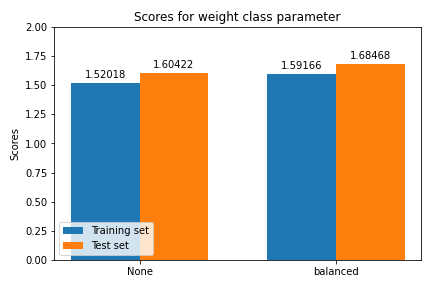
\includegraphics[width=1\linewidth]{images/2-LBM-model_weight_class.png}}
    \captionsetup{width=0.85\linewidth}
    \captionsetup{justification=centering}
    \caption{Average multi-class Log Loss score over 10 iterations.}
    \label{fig:2-LBM-model_weight_class}
\end{figure}

%------------------------------------

\section*{Linear baseline model - fit intercept parameter}

\begin{figure}[H]
    \fbox{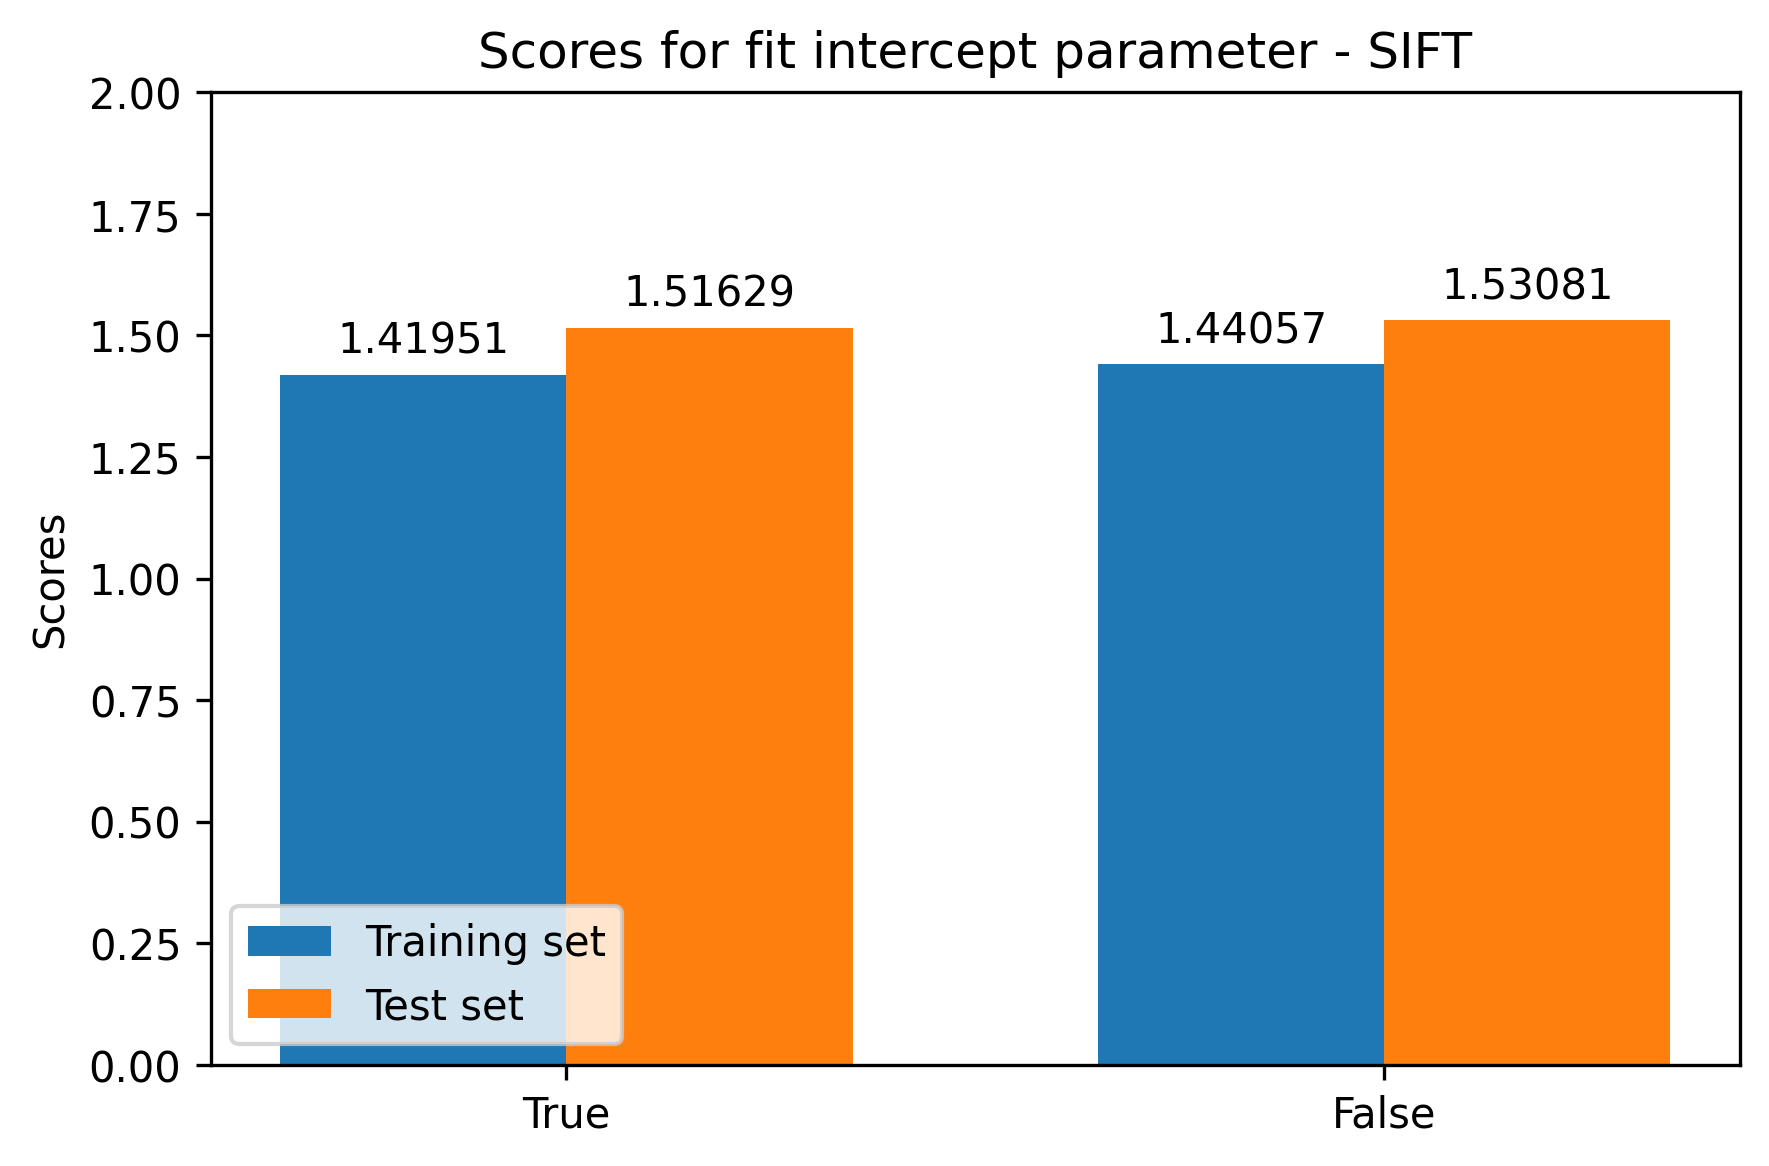
\includegraphics[width=1\linewidth]{images/2-LBM-model_fit_intercept.png}}
    \captionsetup{width=0.85\linewidth}
    \captionsetup{justification=centering}
    \caption{Average multi-class Log Loss score over 5 iterations.}
    \label{fig:2-LBM-model_fit_intercept}
\end{figure}

%references list
\nocite{*}
\printbibliography[heading=bibintoc, title={References}]
\end{document}
